\begin{frame}{Git Objects}
Each Git object has its own hash value and is
stored in .git/objects/FOLDER/FILE,
where FOLDER is the first two digit of its hash value
and the FILE Is the rest of its 38 digits. Git has 4 types of objects
\begin{enumerate}
\item\textbf{commit}: is created upon each commiting and contains a tree object, parent, author, commiter
and a message.
\item \textbf{tree}: is similar to directory in UNIX and is indeed staging area (index) and contains 
blobs and sub-trees. 
\item \textbf{blob} (binary large object): is the file content without
file name. 
\item\textbf{tag} (annotated)
\end{enumerate}
\end{frame}

\begin{frame}{Git Objects}
  \begin{figure}
    \begin{center}
    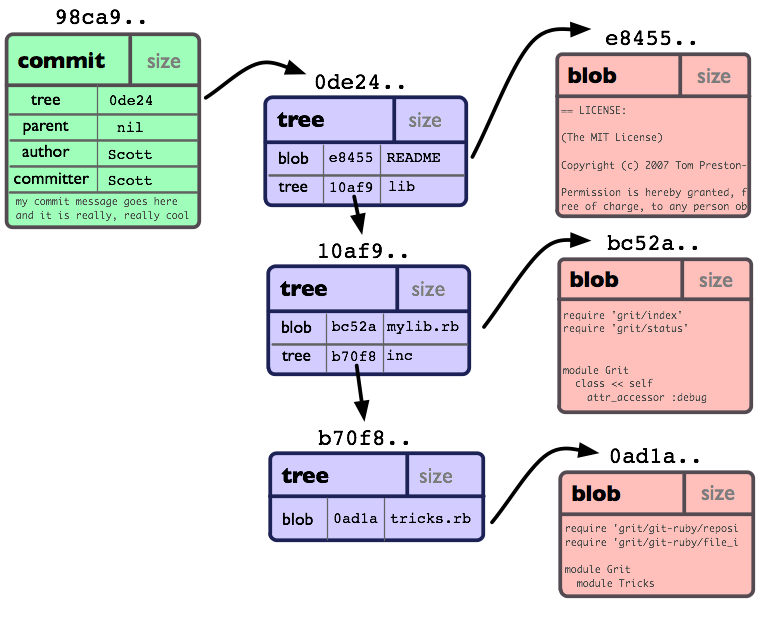
\includegraphics[width=0.8\linewidth]{pics/objects.png}
    \vspace{-0.3cm}
    \caption{\footnotesize Commit, tree and blob objects (Source: https://shafiul.github.io)}
  \end{center}
\end{figure}
\end{frame}

\begin{frame}{Git Objects}
  \begin{itemize}
      \item Create hash object
        \comm{git hash-object -w FILE} (-w stands for write. If given, saves the hash .git/objects. If not given only shows the hash)
        \comm{echo "hello" | git hash-object \dhyphen stdin -w} (created hash from standard input)
      \comm{git cat-file -t HASH} (shows the type of hash value)
      \comm{git cat-file -p HASH} (shows the content of hash value)
      \comm{git cat-file -p BRANCH\textasciicircum\{tree\}} (shows the content of tree, i.e., blobs and sub-trees, of the tip of the given branch)
      \comm{git cat-file -p HASH\textasciicircum\{tree\}} (shows the content of tree, i.e., blobs and sub-trees, of the tip of the given hash)
  \end{itemize}
\end{frame}
\begin{frame}{Git Objects}{Add, Commit in low level Git}
      This examples shows how to create, add and commit changes into
      git, without using "git add" and "git commit" commands.   
      \begin{itemize}
    \item We add one line, i.e., "hello", to the FILE (any given file) and commit it.

          \comm{echo "hello" >> FILE} (adds "hello" to the end FILE)
          \comm{git hash-object FILE -w} (outputs a hash which is used below, i.e., HASH)
      \comm{git update-index \dhyphen add \dhyphen cacheinfo 100644 HASH FILE} (adds the changes to FILE to a new staging area)
      \comm{git write-tree} (writes the staging area out to a tree object and creates a tree object with a TREE-HASH)
          \comm{git commit-tree -p PARENT-HASH -m "MESSAGE" TREE-HASH} (does what git commit -m "MESSAGE" does)
  \end{itemize}
\end{frame}

